% !TEX root = ../../main.tex

\section{Calorimetry dataset UiO-66(Zr)}

\begin{figure}[htb]
    \centering

    \begin{subfigure}{0.20\linewidth}
        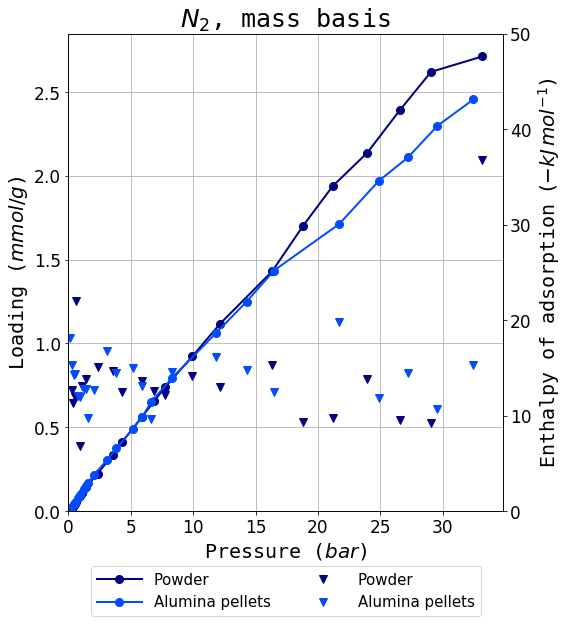
\includegraphics[width=\textwidth]{calo/UiO-66(Zr)/N2-mass-basis-iso}%
        \label{appx:fgr:shaping:uio66n2mass}
    \end{subfigure}%
    \begin{subfigure}{0.20\linewidth}
        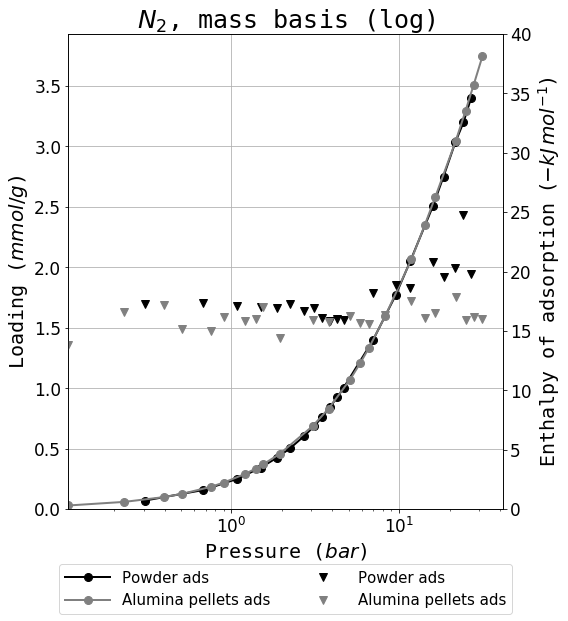
\includegraphics[width=\textwidth]{calo/UiO-66(Zr)/N2-mass-basis-log-iso}%
        \label{appx:fgr:shaping:uio66n2masslog}
    \end{subfigure}%
    \begin{subfigure}{0.20\linewidth}
        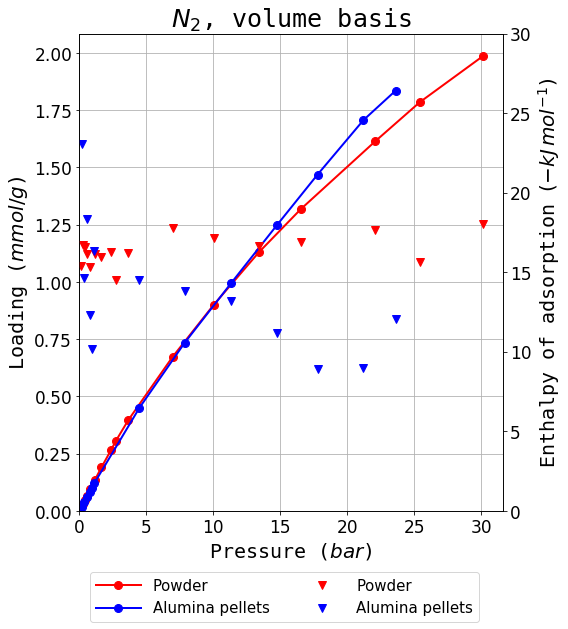
\includegraphics[width=\textwidth]{calo/UiO-66(Zr)/N2-volume-basis-iso}%
        \label{appx:fgr:shaping:uio66n2volume}
    \end{subfigure}%
    \begin{subfigure}{0.20\linewidth}
        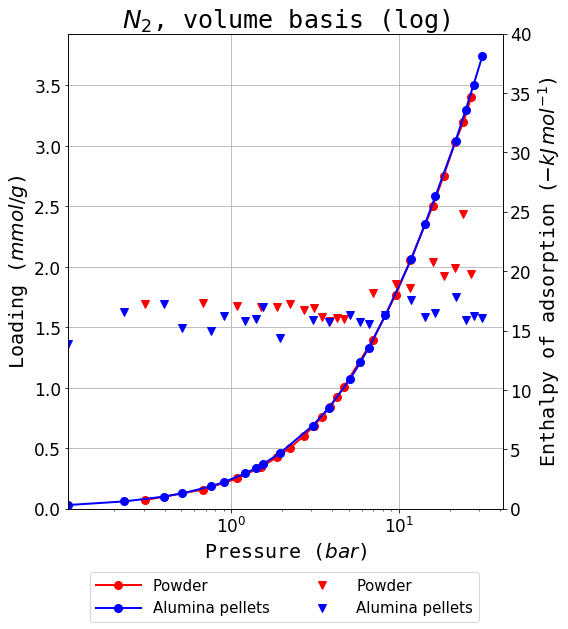
\includegraphics[width=\textwidth]{calo/UiO-66(Zr)/N2-volume-basis-log-iso}%
        \label{appx:fgr:shaping:uio66n2volumelog}
    \end{subfigure}%
    \begin{subfigure}{0.20\linewidth}
        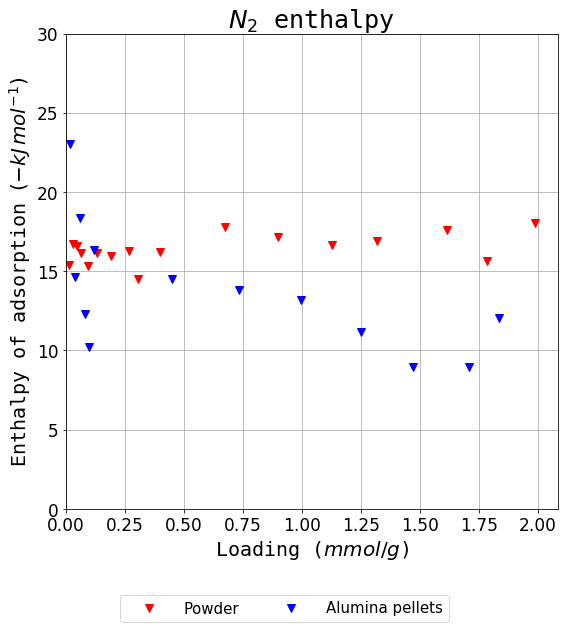
\includegraphics[width=\textwidth]{calo/UiO-66(Zr)/N2-enth}%
        \label{appx:fgr:shaping:uio66n2enth}%
    \end{subfigure}%
    

    \begin{subfigure}{0.20\textwidth}
        \includegraphics[width=\textwidth]{calo/UiO-66(Zr)/co2-mass-basis-iso}%
        \label{appx:fgr:shaping:uio66co2mass}
    \end{subfigure}%
    \begin{subfigure}{0.20\textwidth}
        \includegraphics[width=\textwidth]{calo/UiO-66(Zr)/co2-mass-basis-log-iso}%
        \label{appx:fgr:shaping:uio66co2masslog}
    \end{subfigure}%
    \begin{subfigure}{0.20\textwidth}
        \includegraphics[width=\textwidth]{calo/UiO-66(Zr)/co2-volume-basis-iso}%
        \label{appx:fgr:shaping:uio66co2volume}
    \end{subfigure}%
    \begin{subfigure}{0.20\textwidth}
        \includegraphics[width=\textwidth]{calo/UiO-66(Zr)/co2-volume-basis-log-iso}%
        \label{appx:fgr:shaping:uio66co2volumelog}
    \end{subfigure}%
    \begin{subfigure}{0.20\textwidth}
        \includegraphics[width=\textwidth]{calo/UiO-66(Zr)/co2-enth}%
        \label{appx:fgr:shaping:uio66co2enth}%
    \end{subfigure}%


    \begin{subfigure}{0.20\textwidth}
        \includegraphics[width=\textwidth]{calo/UiO-66(Zr)/co-mass-basis-iso}%
        \label{appx:fgr:shaping:uio66comass}
    \end{subfigure}%
    \begin{subfigure}{0.20\textwidth}
        \includegraphics[width=\textwidth]{calo/UiO-66(Zr)/co-mass-basis-log-iso}%
        \label{appx:fgr:shaping:uio66comasslog}
    \end{subfigure}%
    \begin{subfigure}{0.20\textwidth}
        \includegraphics[width=\textwidth]{calo/UiO-66(Zr)/co-volume-basis-iso}%
        \label{appx:fgr:shaping:uio66covolume}
    \end{subfigure}%
    \begin{subfigure}{0.20\textwidth}
        \includegraphics[width=\textwidth]{calo/UiO-66(Zr)/co-volume-basis-log-iso}%
        \label{appx:fgr:shaping:uio66covolumelog}
    \end{subfigure}%
    \begin{subfigure}{0.20\textwidth}
        \includegraphics[width=\textwidth]{calo/UiO-66(Zr)/co-enth}%
        \label{appx:fgr:shaping:uio66coenth}%
    \end{subfigure}%


    \begin{subfigure}{0.20\textwidth}
        \includegraphics[width=\textwidth]{calo/UiO-66(Zr)/ch4-mass-basis-iso}%
        \label{appx:fgr:shaping:uio66ch4mass}
    \end{subfigure}%
    \begin{subfigure}{0.20\textwidth}
        \includegraphics[width=\textwidth]{calo/UiO-66(Zr)/ch4-mass-basis-log-iso}%
        \label{appx:fgr:shaping:uio66ch4masslog}
    \end{subfigure}%
    \begin{subfigure}{0.20\textwidth}
        \includegraphics[width=\textwidth]{calo/UiO-66(Zr)/ch4-volume-basis-iso}%
        \label{appx:fgr:shaping:uio66ch4volume}
    \end{subfigure}%
    \begin{subfigure}{0.20\textwidth}
        \includegraphics[width=\textwidth]{calo/UiO-66(Zr)/ch4-volume-basis-log-iso}%
        \label{appx:fgr:shaping:uio66ch4volumelog}
    \end{subfigure}%
    \begin{subfigure}{0.20\textwidth}
        \includegraphics[width=\textwidth]{calo/UiO-66(Zr)/ch4-enth}%
        \label{appx:fgr:shaping:uio66ch4enth}%
    \end{subfigure}%

    \caption{Complete isotherm and enthalpy dataset for UiO-66(Zr)}
\end{figure}
\begin{figure}[htb]\ContinuedFloat%

    \begin{subfigure}{0.20\textwidth}
        \includegraphics[width=\textwidth]{calo/UiO-66(Zr)/c2h6-mass-basis-iso}%
        \label{appx:fgr:shaping:uio66c2h6mass}
    \end{subfigure}%
    \begin{subfigure}{0.20\textwidth}
        \includegraphics[width=\textwidth]{calo/UiO-66(Zr)/c2h6-mass-basis-log-iso}%
        \label{appx:fgr:shaping:uio66c2h6masslog}
    \end{subfigure}%
    \begin{subfigure}{0.20\textwidth}
        \includegraphics[width=\textwidth]{calo/UiO-66(Zr)/c2h6-volume-basis-iso}%
        \label{appx:fgr:shaping:uio66c2h6volume}
    \end{subfigure}%
    \begin{subfigure}{0.20\textwidth}
        \includegraphics[width=\textwidth]{calo/UiO-66(Zr)/c2h6-volume-basis-log-iso}%
        \label{appx:fgr:shaping:uio66c2h6volumelog}
    \end{subfigure}%
    \begin{subfigure}{0.20\textwidth}
        \includegraphics[width=\textwidth]{calo/UiO-66(Zr)/c2h6-enth}%
        \label{appx:fgr:shaping:uio66c2h6enth}%
    \end{subfigure}%


    \begin{subfigure}{0.20\textwidth}
        \includegraphics[width=\textwidth]{calo/UiO-66(Zr)/c3h8-mass-basis-iso}%
        \label{appx:fgr:shaping:uio66c3h8mass}
    \end{subfigure}%
    \begin{subfigure}{0.20\textwidth}
        \includegraphics[width=\textwidth]{calo/UiO-66(Zr)/c3h8-mass-basis-log-iso}%
        \label{appx:fgr:shaping:uio66c3h8masslog}
    \end{subfigure}%
    \begin{subfigure}{0.20\textwidth}
        \includegraphics[width=\textwidth]{calo/UiO-66(Zr)/c3h8-volume-basis-iso}%
        \label{appx:fgr:shaping:uio66c3h8volume}
    \end{subfigure}%
    \begin{subfigure}{0.20\textwidth}
        \includegraphics[width=\textwidth]{calo/UiO-66(Zr)/c3h8-volume-basis-log-iso}%
        \label{appx:fgr:shaping:uio66c3h8volumelog}
    \end{subfigure}%
    \begin{subfigure}{0.20\textwidth}
        \includegraphics[width=\textwidth]{calo/UiO-66(Zr)/c3h8-enth}%
        \label{appx:fgr:shaping:uio66c3h8enth}%
    \end{subfigure}%

    \begin{subfigure}{0.20\textwidth}
        \includegraphics[width=\textwidth]{calo/UiO-66(Zr)/c3h6-mass-basis-iso}%
        \label{appx:fgr:shaping:uio66c3h6mass}
    \end{subfigure}%
    \begin{subfigure}{0.20\textwidth}
        \includegraphics[width=\textwidth]{calo/UiO-66(Zr)/c3h6-mass-basis-log-iso}%
        \label{appx:fgr:shaping:uio66c3h6masslog}
    \end{subfigure}%
    \begin{subfigure}{0.20\textwidth}
        \includegraphics[width=\textwidth]{calo/UiO-66(Zr)/c3h6-volume-basis-iso}%
        \label{appx:fgr:shaping:uio66c3h6volume}
    \end{subfigure}%
    \begin{subfigure}{0.20\textwidth}
        \includegraphics[width=\textwidth]{calo/UiO-66(Zr)/c3h6-volume-basis-log-iso}%
        \label{appx:fgr:shaping:uio66c3h6volumelog}
    \end{subfigure}%
    \begin{subfigure}{0.20\textwidth}
        \includegraphics[width=\textwidth]{calo/UiO-66(Zr)/c3h6-enth}%
        \label{appx:fgr:shaping:uio66c3h6enth}%
    \end{subfigure}%


    \begin{subfigure}{0.20\textwidth}
        \includegraphics[width=\textwidth]{calo/UiO-66(Zr)/c4h10-mass-basis-iso}%
        \label{appx:fgr:shaping:uio66c4h10mass}
    \end{subfigure}%
    \begin{subfigure}{0.20\textwidth}
        \includegraphics[width=\textwidth]{calo/UiO-66(Zr)/c4h10-mass-basis-log-iso}%
        \label{appx:fgr:shaping:uio66c4h10masslog}
    \end{subfigure}%
    \begin{subfigure}{0.20\textwidth}
        \includegraphics[width=\textwidth]{calo/UiO-66(Zr)/c4h10-volume-basis-iso}%
        \label{appx:fgr:shaping:uio66c4h10volume}
    \end{subfigure}%
    \begin{subfigure}{0.20\textwidth}
        \includegraphics[width=\textwidth]{calo/UiO-66(Zr)/c4h10-volume-basis-log-iso}%
        \label{appx:fgr:shaping:uio66c4h10volumelog}
    \end{subfigure}%
    \begin{subfigure}{0.20\textwidth}
        \includegraphics[width=\textwidth]{calo/UiO-66(Zr)/c4h10-enth}%
        \label{appx:fgr:shaping:uio66c4h10enth}%
    \end{subfigure}%

    \caption{Complete isotherm and enthalpy dataset for UiO-66(Zr)}%
    \label{appx:fgr:shaping:calouio66}
\end{figure}
